\documentclass[12 pt]{article}
\usepackage{hyperref}
\usepackage{fancyhdr}
\usepackage{setspace}
\usepackage{enumerate}
\usepackage{amsmath}
\usepackage{lastpage}
\usepackage{mathtools,float}
\usepackage{tikz}
\usepackage{tabularx}
\usepackage{ltablex}
\usepackage{amssymb}
\usepackage{textcomp}
\usepackage[T1]{fontenc}
\usepackage{listings}
\usepackage[margin=1 in]{geometry}
\allowdisplaybreaks
%\usepackage[dvipsnames]{xcolor}   %May be necessary if you want to color links
\hypersetup{
	%colorlinks=true, %set true if you want colored links
	linktoc=all,     %set to all if you want both sections and subsections linked
	linkcolor=black,  %choose some color if you want links to stand out
}
\usepackage{graphicx}
\graphicspath{{Images/}}
\author{Julian Lore}
\date{Last updated: \today}
\title{COMP 206: Intro to Software Systems Review}
\pagestyle{fancy}
\lhead{COMP 206}
\chead{\leftmark}
\rhead{Julian Lore}
\cfoot{Page \thepage \ of \pageref{LastPage}}
\newcommand{\tab}[1]{\hspace{.2\textwidth}\rlap{#1}}
\begin{document}
	\onehalfspacing
	\maketitle
	Adapted from Joseph Vybihal's Winter 2017 COMP206 slides.
	\tableofcontents
	\section{Software Systems}
	\subsection{What is a Software System?} 
	A \textbf{system} has several parts. By themselves, not special. They cooperate together to make something. Addition of several sub-systems (programs that depend on other programs). System is the complete application that interacts directly with user.
	\\
	A \href{https://en.wikipedia.org/wiki/Software_system}{software system} consists of a system with components (based on software) that form a part of a computer system. I.e. has separate programs, config files, documentation. Single components from a software system are usually useless without each other.
	\\ In this class, our programs will send instructions to the operating system, which will deal with sending stuff to the actual hardware.
	\subsection{Examples of Software Systems}
	\paragraph{Email} Email clients don't know how to send email, they just send data through a wire. Keeps sending it to the next person (connected in network), until finally ISP or something else knows what to do with the email. Each piece only knows so much, all have to be together to work. 
	\paragraph{Facebook}
	Needs Internet, ISP, PC/phone/browser and then the server/application/database. With only one thing, wouldn't be able to use Facebook.
	\paragraph{Object oriented programming/Java} Requires JVM, computer, etc. Text file $\to$ byte code converter $\to$ JVM $\to$ Libs $\to$ OS $\to$ PC $\to$GPU or Network$\to$Internet
	\paragraph{Internet} The Internet is the quintessential software system! Has many sub-systems, such as:
	\begin{itemize}
		\item Local PC
		\item Server
		\item Network
		\item Encryption
		\item etc.
	\end{itemize} See 1.4 For more information.
	\subsection{Operating Systems}
	\paragraph{Drivers} Small pieces of software, allow external devices to communicate with PC generically. So application does not have to deal separately with all different types of hardware.
	\paragraph{What is an Operating System?} Piece of software, allows users to use computer without knowing inner workings. Main use is to manage resources, execute programs properly. Middle man between low-level hardware \& users/programs. Also provides libraries.
	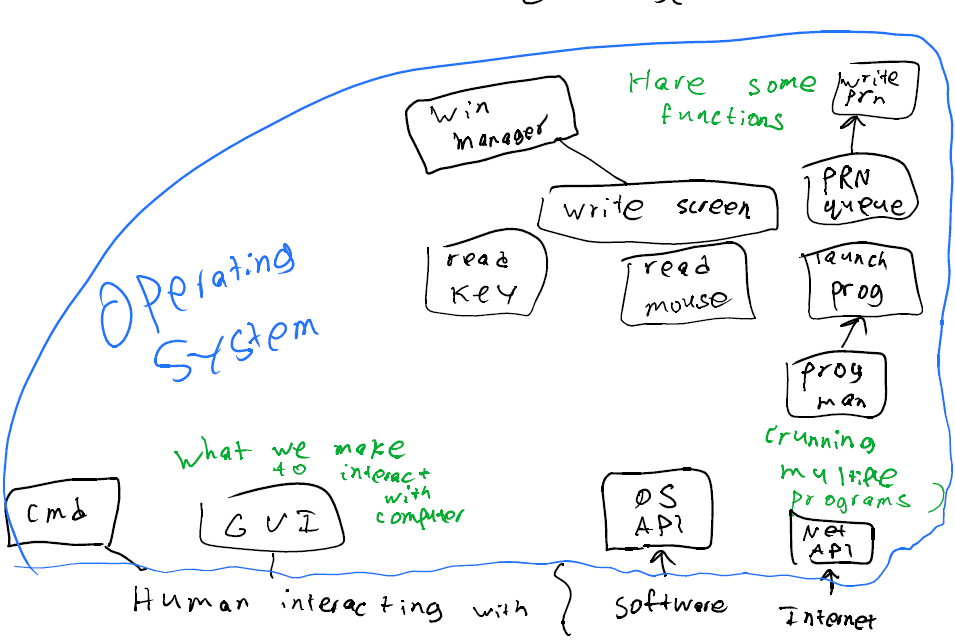
\includegraphics[scale=0.5]{os}
	\paragraph{OS Architecture}
	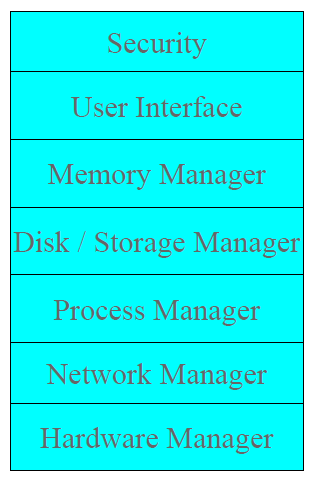
\includegraphics[scale=0.5]{oss} Uses ideas from systems and subsystems.
	\begin{itemize}
		\item Security 
		\begin{itemize}
			\item Passwords
			\item Encryption
			\item File permissions
		\end{itemize}
		\item User Interface
		\begin{itemize}
			\item GUI, CLI, Shell memory
		\end{itemize}
		\item Memory Manager
		\begin{itemize}
			\item Find memory for programs
			\item Format RAM
			\item Manage cache, buffers, spools
		\end{itemize}
		\item Storage Manager
		\begin{itemize}
			\item Secondary Storage
			\item Floppy disks
			\item Hard disks
			\item Memory sticks
			\item etc.
		\end{itemize}
		\item Process Manager
		\begin{itemize}
			\item Runs programs
			\item Multi-processing/multi-CPU
			\item Kills programs
			\item Run-time errors
		\end{itemize}
		\item Network Manager
		\begin{itemize}
			\item LAN
			\item Internet
			\item etc.
		\end{itemize}
		\item Hardware Manager
		\begin{itemize}
			\item Drivers
			\item Assembler \& registers
			\item etc.
		\end{itemize}
	\end{itemize}
	\subsection{Internet} All interconnected computers around the world. 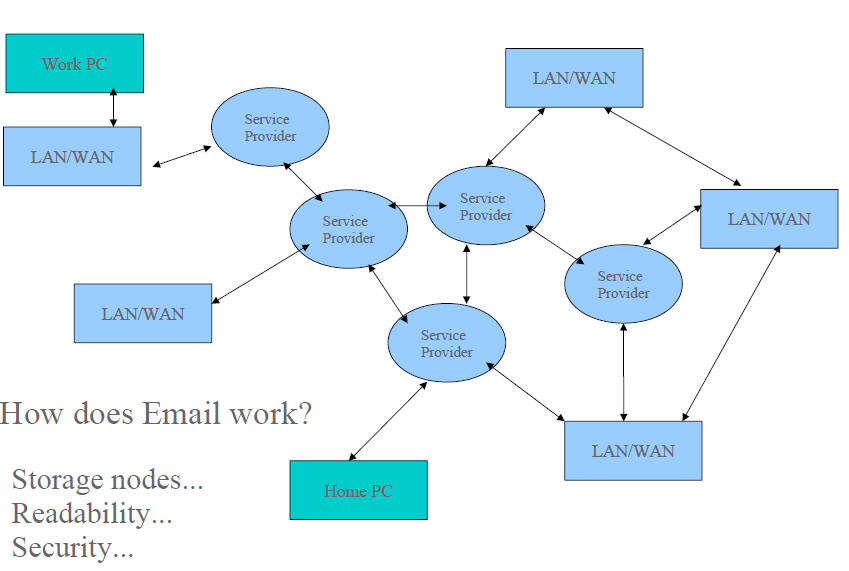
\includegraphics[scale=0.5]{inter}
	\subparagraph{What is a Network?}
	Wire, permits communication between computers. \textbf{LAN:} Local Area Network, computers in same room/building. \textbf{WAN:} Wide Area Network, computers in different buildings/cities, more than 1 server interconnecting big network nodes.
	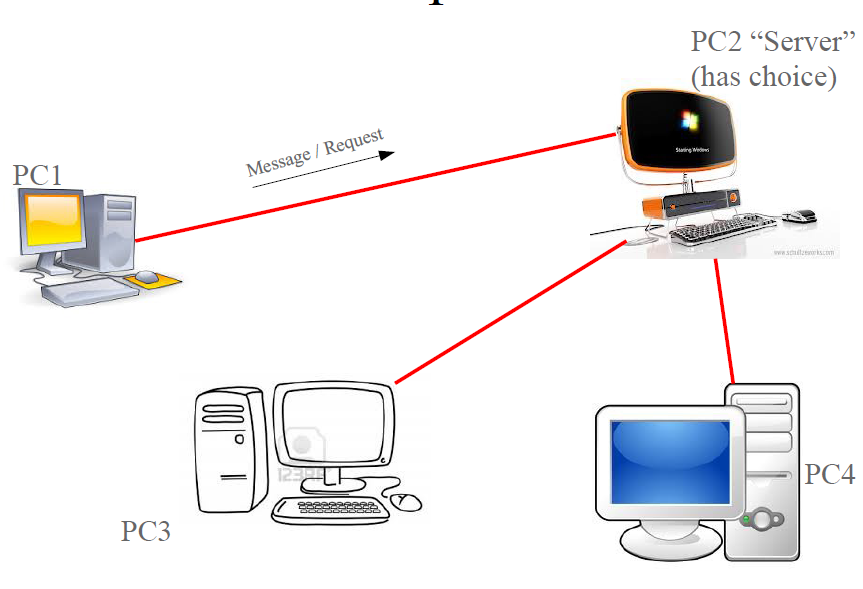
\includegraphics[scale=0.4]{ntw}
	\paragraph{Client/Server}
	\begin{itemize}
		\item Client sends request packet to server
		\item Server tries to find requested thing
		\item Server sends reply packet with data/program
		\item Client copies into memory and executes
	\end{itemize}
	Programs run on client, but programs stored on server, data is spread out. \textbf{MasterComputer/Main frame} is the opposite, programs stored \& run on server, client just sees it.
	Additional terms: \textbf{Handshaking} consists of agreeing on packet format \& passwords. \textbf{Comm-error}, packet lost, resend request or time-out. 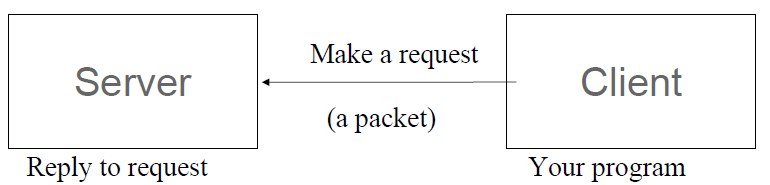
\includegraphics[scale=0.3]{cs}
	\paragraph{Service Providers} Special server, knows locations of other servers on the Internet. Uses this knowledge to deliver package to right destination. Internet = WAN of service providers that are connected to independent LAN \& WAN networks.
	\paragraph{Web} Subset of Internet with only interconnected ISP servers. Interacts solely with browsers.
	\paragraph{Public\_HTML} Servers connected to Internet have a directory/folder called public\_html, which is public. By default, only this is accessible from Browser. The default operation for the Internet is to display folders and files at that Internet address (like a file-browser), like \href{https://www.kernel.org/pub/software/scm/git/}{this}. Need an index.html or other stuff to change default behavior and display a ``web page".
	\paragraph{Communicating with Other Computers} Each computer needs a unique ID, today we use our \textbf{IP Address} as our unique ID number. 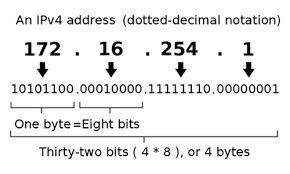
\includegraphics{ipv4}
	\section{Unix}
	\subsection{About Unix}
	\paragraph{History}
	Failed OS by AT\&T Bell Laboratories called Multics, $1^{st}$ OS with 2 windows \& 2 programs at the same time. Ken Thompson was working on project, writing game called \textit{Space Travel}. Ported game to PDP-7 when project was canceled. Wrote Unix to make it easier to port. 3 types: System V UNIX (based off original), BSD UNIX (based on Berkeley Software Distribution) and UNIX-like (behave like UNIX, includes \textbf{Linux}, which we'll be using).
	\paragraph{General Info} Unix is:
	\begin{itemize}
		\item Optimized/simple
		\item Password-based security
		\item Driven by command line
		\item Client-server
		\end{itemize}
		Unix is client/server! Companies buy one huge machine (server) and many small terminals (client). Can SSH into a SOCS machine at school.
	\paragraph{OS Components} Unix is a modular OS. 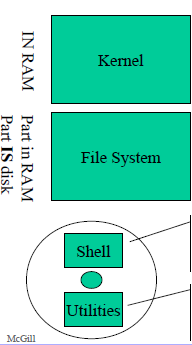
\includegraphics[scale=0.6]{osc} Several components: 
	\begin{itemize}
		\item Kernel
		\begin{itemize}
			\item In RAM
			\item Handles logging in
			\item Task switching
			\item Manages everything
			\item Basic interface
			\item Drivers, run-time stack
		\end{itemize}
		\item File System
		\begin{itemize}
			\item How is disk drive formatted
			\item FAT (File Allocation Table)
			\item Data structure making files "real"
			\item Everything is a "Program"
			\item R/w to disk \& peripherals
		\end{itemize}
		\item Shell
		\begin{itemize}
			\item More advanced UI
			\item Global memory
			\item Commands to interact with shell
		\end{itemize}
		\item Utilities
		\begin{itemize}
			\item Extra commands and programs
			\item Drivers
		\end{itemize}
		%\textbf{Session} consists of Kernel $\to$ File System $\to$ login until logout
	\end{itemize}
	\paragraph{Users} Need an account on a Unix machine to use it. Consists of a user name and password. User gets a \textbf{home directory} ($\sim$). Accounts are members of at least one group. Groups used for permission purposes. Every Unix machine has a \textbf{root} account, with ALL permissions.
	\paragraph{Passwords} Since all Unix security is based on passwords, important to have a good password. Breach consists of someone else logging in with your password. Shouldn't use dictionary words because there are dictionary attacks. Other attacks include getting to know the user and brute force. Want a mix of upper and lower case, numbers, punctuation.
	\subsection{Sessions} 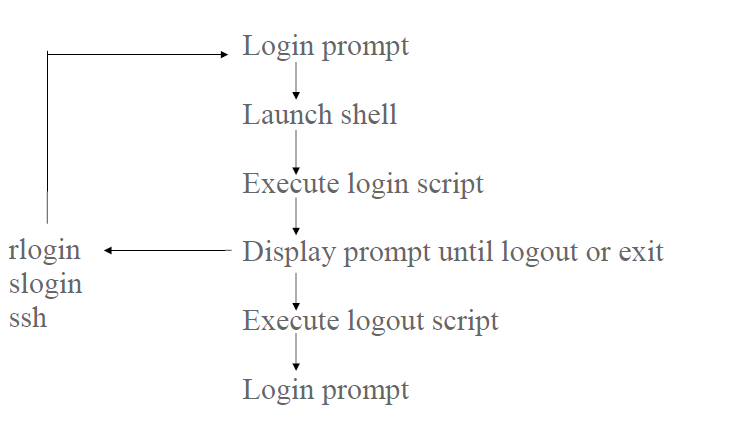
\includegraphics[scale=0.5]{ses} One session goes from login, loops the prompt many times until you logout. rlogin, slogin, ssh used to create another session within a login.
	\paragraph{Environment Session Memory} Has stuff like user name, home, shell, etc.
	\\ When you start the shell, OS sets up environment, a collection of variables which can be accessed from any application launched from that environment. env \& set show you current environment variables. setenv and set are not used in bash to change an environment variable in Bash, just write var=value. Echo can give you specific env variables, like echo \$var.
	\section{Bash/Command-line} 
	\paragraph{Command-line Prompt}Basically a while look that keeps reading the input you give it until you logout or exit.
	\paragraph{Syntax} Program -switches arguments
	\\ Program is any command or executable. Switches are parameters that modify program's execution, arguments are fed to program. 
	\subsection{Good Commands to Know}
	\begin{tabularx}{\textwidth}{|X|X|X|X|}
		\hline
		Command & Switches/Args & Examples & Usage
		\\\hline
		 ls & -l (long output) & ls ; ls -l ; ls text.txt & lists files and directories
		 \\ & -a (all, hidden) [file/dir] & &
		\\\hline
		 whoami &&& Tells you user logged in as
		 \\\hline
		 who &&& Who is logged on server
		 \\\hline
		 exit &&& exits shell
		 \\\hline 
		 logout &&& logs out of session, can logout of a nested session
		 \\\hline
		 finger & username@host & finger jlore & info on user
		 \\\hline
		 ssh & username@host & ssh jlore@mimi.cs.mcgill.ca & ssh into this user
		 \\\hline
		 mkdir & directoryname & mkdir test & make directory
		 \\\hline 
		 cp & filename destination file & cp a.txt b.txt ; cp a.txt /jl & copy a file
		 \\\hline
		 cd & [directory] [..] & cd test ; cd .. (goes up 1 dir) ; cd (goes home) & change dir
		 \\\hline
		 cat & file & cat test.txt & reads text, concatenates files, can read 2 at once
		 \\\hline
		 rm & file & rm test.txt & removes a file
		 %\\\hline
		 %more & & & paginates text
		 \\\hline
		 sort & -(reverse alphabetical) && sorts text alphabetically
		 \\\hline
		 pwd & && prints working directory
		 \\\hline 
		 rmdir & directory & rm test & removes EMPTY directory
		 \\\hline 
		 chgrp & group file & chgrp friends test.txt & changes group of file
		 \\\hline
		 chmod & u(user)g(group)a(all) & chmod u=r test.txt & change permissions
		 \\ ~&  +(adds perm)-(removes)=(replaces) rwx 421 file &  (changes user to read) &
		 \\ &(0=no perm 1=exec) & chmod 000 test.txt&
		 \\ &(2=write 4=read)& &
		 \\\hline 
		 chown & owner file & chown jlore test.txt & changes owner of file
		 \\\hline
		 mv & file1 file2 & mv test.txt /jlore/test.txt & moves file1 into file2
		 \\\hline 
		 echo & text/string & echo hi & echoes string to stdout
		 \\\hline 
		 head & [-number] file & head -2 test & display first n or first few (if no number) lines of file
		 \\\hline
		 tail & [-number] file & tail -2 test & display last n or last few lines of file
		 \\\hline 
		 more & file & more test & page through file, enter advances a page
		 \\\hline 
		 less & file & less test & navigate through paginated file, better than more
		 \\\hline 
		 man & command/program & man ls & get manual page for a program
		 \\\hline
		 date & [options] & & gets current date \& time
		 \\\hline 
		 du & [options] [dir/file] & du source/ & shows disk space usage
		 \\\hline 
		 hostname &&& Gives name of machine
		 \\\hline 
		 uname & [option] && Prints system info
		 \\\hline 
		 script & file & script record.txt & Records everything appearing on screen (IN/OUT) to file until exit or ctrl-D
		 \\\hline 
		 which & command & which ls & Shows path where command is located
		 \\\hline
		 kill & [options] [-SIGNAL] [pid\#] & kill -9 1234 & Kills a process id, -9 is sigkill, aggressive/forceful kill
		 \\\hline 
		 ps & [options] -a (all processes/users) -e (environment) -g (group leaders too) -l (long) -u (shows user, also more info like \% resources) -x (includes things not run from terms) -f (full)& ps -a & Shows status of active processes
		 \\\hline 
		 top & && Monitors resource usage of active processes
		 \\\hline
		 tar & -c (create new) -r (update) -x (extract) -f (archive name) -v (verbose) -z (compress using gzip) (files/dir)& tar -cvf log.tar *.log ; tar -zcvf log.tgz *.log ; tar -xvf log.tar /tmp/log & Archive manipulation using tar, see 3.2
		 \\\hline
		 diff & [op] file1 file2 & diff text text2 & compares 2 files
		 \\\hline
		 file & [op] file & file text & What ``kind" of file?
		 \\\hline
		 find & [op] [path] expressions & find test & Finds files matching pattern
		 \\\hline
		 ln & -s (soft link) source target & ln fav.txt read & Links source to target. Default is hard link, gives another name to a file. Soft/symbolic link is an indirect pointer, does not affect target file.
		 \\\hline
		 paste & [op] file1 file2 & paste text1 text2 & combines 2 files, one after other
		 \\\hline
		 touch & [op] [date] file & touch text & Create empty file or update access time
		 \\\hline
		 wc & [op] file(s) & wc text & word count
		 \\\hline
		 write & userid & write jlore & Sends text message to someone \textasciicircum D to end, mesg -y/n to turn on/off
		 \\\hline
		 wall &&& write to all
		 \\\hline
		 grep & [op] -i (ignore case) -c (return only count of matches) -v (invert, display ones that don't match) -n (adds line number of match) -l (filenames of matches) string files & grep hi text & Search for occurrences of String, supports regex
		 \\\hline
		 sed & [op] -i (interactive, update current file) files & sed -i \textquotesingle 1d \textquotesingle text (deletes first line) ; sed -i \textquotesingle 1iHello \textquotesingle text (inserts Hello at 1st line) & stream editor
		 \\\hline
		 awk & [op] files & awk \textquotesingle NR==1\textquotesingle text (reads first line) & scan for patterns in file
		 \\\hline
		 clear &&& clears screen/prompt
		 \\\hline
		 expr & math & expr 1 + 2 & Does integer math
		 \\\hline
	\end{tabularx}
	\paragraph{Common switches (mainly cp, mv, rm)}
	\begin{enumerate}[.]
		\item -i: interactive
		\\ prompt and wait for confirmation
		\item -r or -R: recursive
		\\ visits directory recursively, visits files and subdirs
		\item -f: force
		\\ don't prompt for confirmation, overrides -i
	\end{enumerate}
	\paragraph{Killing}
	\textasciicircum Z (ctrl-Z) forceful kill
	\\\textasciicircum C (ctrl-C) gentle kill
	\subsection{Files \& Directories}
	\paragraph{Hidden Files/Folders}: Start with ., i.e. .config \\ Can be seen with ls -a
	\paragraph{Wild cards}
	~\\\begin{tabular}{c|c}
		* & anything
		\\ ? & any single char 
		\\ $[$abc$]$ & a or b or c
	\end{tabular}
	\paragraph{Directories} Directories are folders. Use same permission system as files. Root denoted by /
	\\ Common Unix system has following directories:
	\begin{itemize}
		\item /etc : config files, pws
		\item /bin : OS executables
		\item /usr : Application installations
		\item /opt : Another application installation dir
		\item /dev : Device files for hardware
		\item /var : Files that vary a lot, like logs
	\end{itemize}
	\paragraph{Typical Directory Structure}~\\
	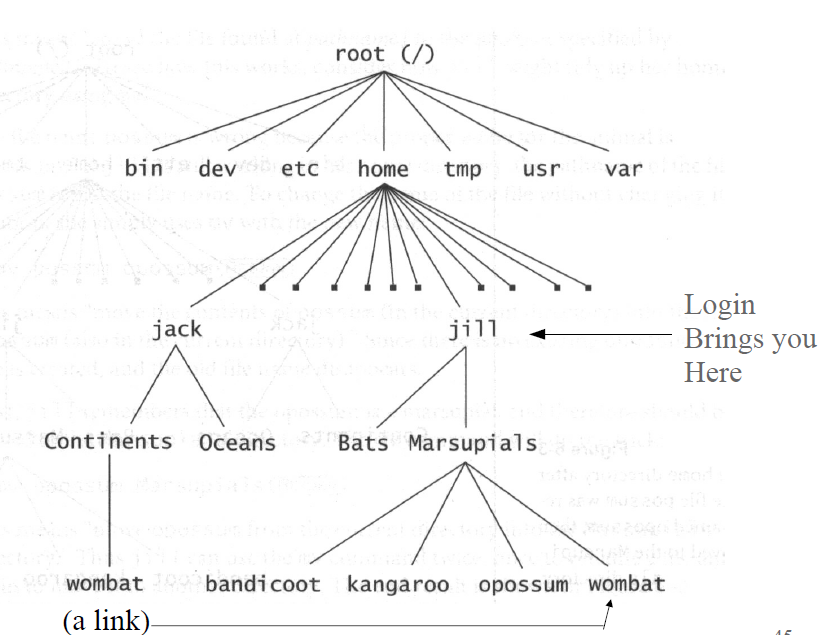
\includegraphics[scale=0.5]{dst}
	\paragraph{Absolute vs Relative Paths}
	\begin{enumerate}[.]
		\item Relative paths: Path from your current directory
		\item Absolute paths: Path from root
		\begin{itemize}
			\item ./folder from current directory, same as folder
			\item ../folder parent directory one up
		\end{itemize}
	\end{enumerate}
	\paragraph{File Descriptors} Created by OS when file opened. Reference to that file. Unix has 3 special file descriptors that are always opened.
	\begin{itemize}
		\item STDIN 0 : keys typed by user gathered here
		\item STDOUT 1 : normal application output sent here
		\item STDERR 2 : where error output is sent
	\end{itemize}
	\paragraph{Permissions}
	Three levels, user, group and other. 3 types of rights, read, write and execute. Can give any combination of these rights to the 3 levels. Permissions usually shown by string of 10 characters, first is if directory or not, then next bunches of 3 are rwx for 3 levels.
		\subparagraph{Directory Listing (ls)}
		Long format: \\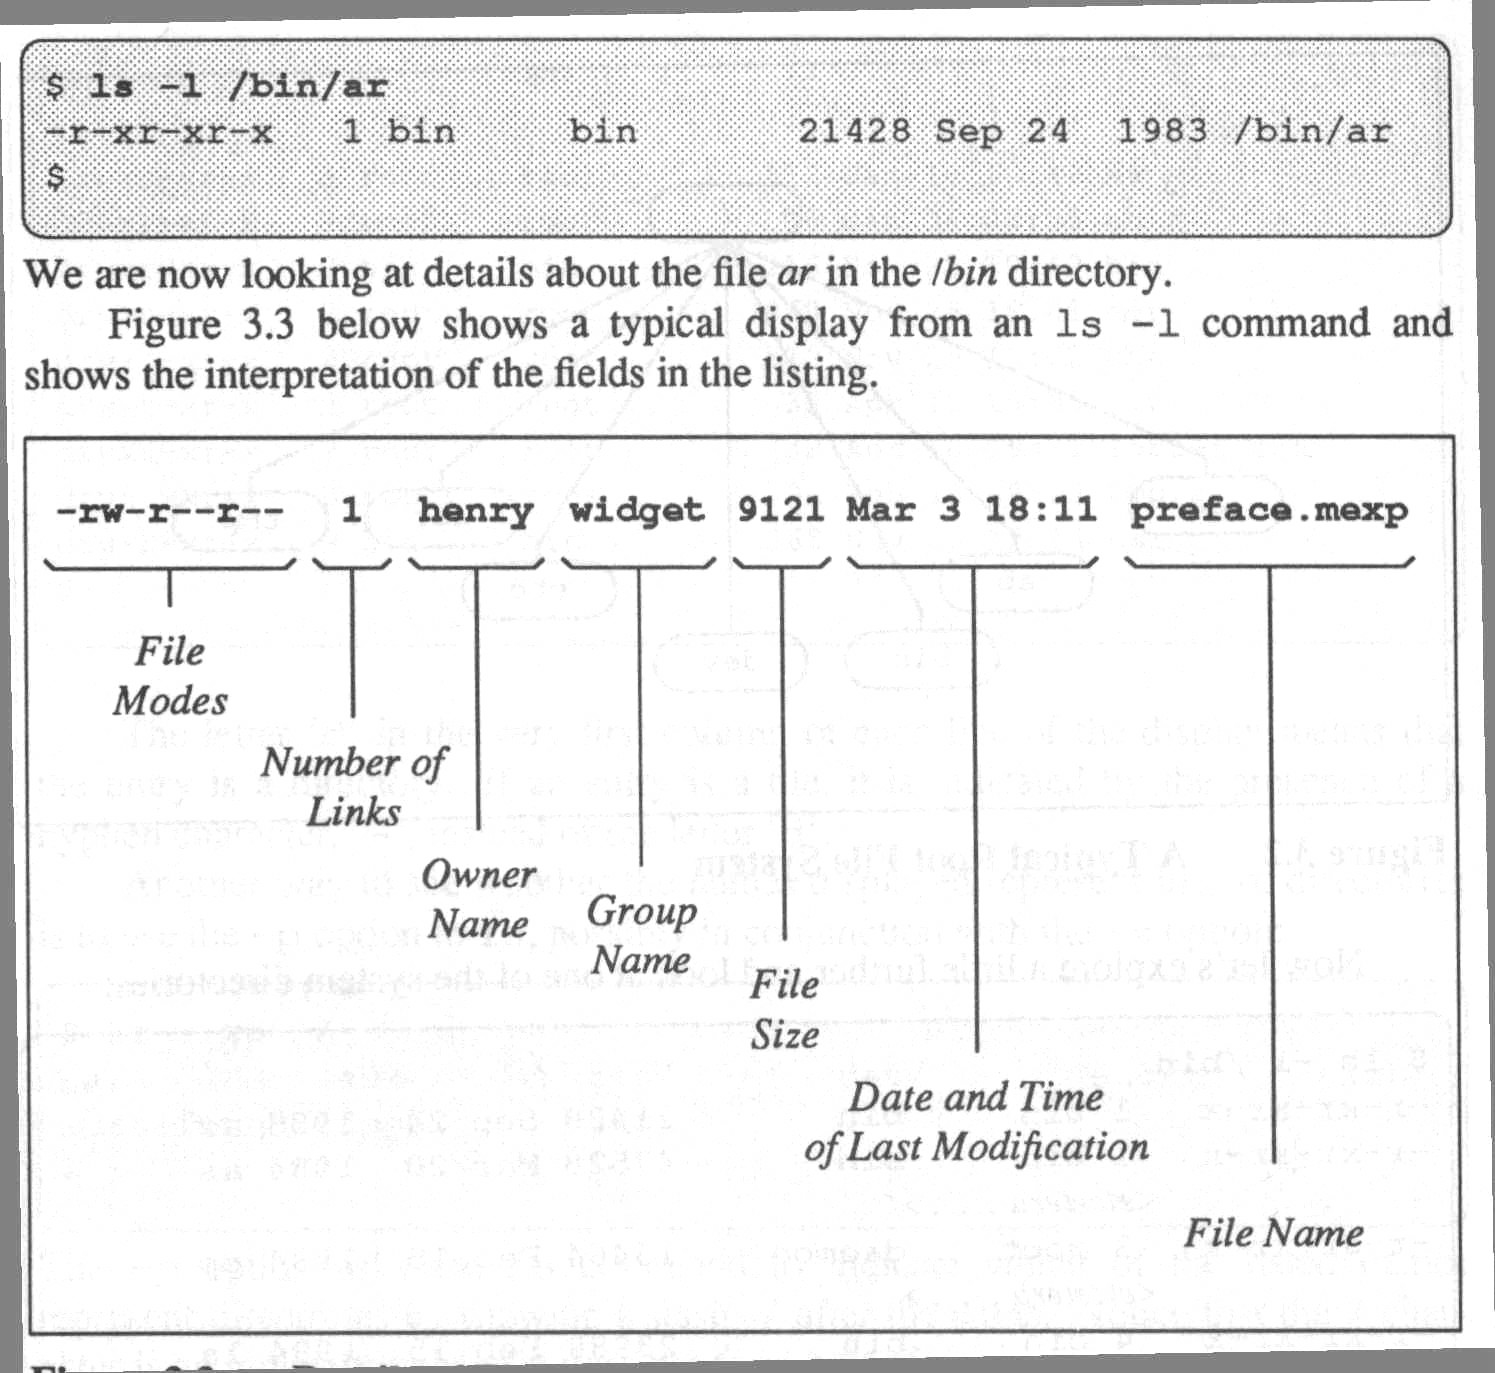
\includegraphics[scale=0.3]{ls}
	\subparagraph{Overlapping} If all/other have rwx, but everyone else has nothing, owner and group cannot rwx, unless the Unix system interprets other as all.
	\paragraph{Archives} TAR, GZIP \& GUNZIP. Archive is a collection of files combined into one file, often compressed. tar combines, gzip compresses. 
	\subsection{Redirection}
	\paragraph{Output} $>$ redirects STDOUT to a text file
	\\ $>>$ appends STDOUT to a text file.
	\paragraph{Input} $<$ takes all input from a file
	\\ To redirect something specific, can prefix by file descriptor, i.e. prog 2$>$errors, redirects errors from prog to errors file.
	\paragraph{Piping/Chaining}
	\begin{enumerate}[.]
		\item Piping commands: redirects STDOUT to another program. i.e. (ls $|$ more) paginates ls output
		\item Doing multiple commands in SUCCESSION: (ls ; echo hi) does ls then echoes hi
		\item Doing multiple commands at ONCE: (ls \& echo hi) does ls and echo at the same time
	\end{enumerate}
	\subsection{Quotes}
	\begin{itemize}
		\item \` \ nested execute symbol \`  \ , executes what's in between first $\to$ string
		\item \textquotesingle as is \textquotesingle 
		\item \textquotedbl pre-process \textquotedbl
		\end{itemize}
	\paragraph{Escape Characters}
	\begin{itemize}
		\item $\backslash$ $\gets$ escape character
		\item $\backslash$n new line
		\item $\backslash$t tab
		\item $\backslash$a bell (noise)
		\end{itemize}
	\subsection{Editors} Command line text editors allow for creation/editing of files at CLI. 
	\begin{itemize}
		\item vi, one of the original ones on Unix, hard to learn. Available on every Unix machine.
		\item pico, simple, based on pine mail client, available on most
		\item emacs, popular, powerful, heavyweight
	\end{itemize}
	There are also graphical text editors.
	\paragraph{Vi}
	Different modes: 
	\begin{itemize}
		\item Edit (i, a, o, O, etc.)
		\begin{itemize}
			\item Edit text
			\item Can press any char
			\item Some vis let you use arrows
		\end{itemize}
		\item Escape Mode (ESC)
		\begin{itemize}
			\item Stops edit
			\item Can use arrow keys
			\item Can use special one letter commands (i,a,h,j,k,l,etc.)
		\end{itemize}
		\item Command Mode (:)
		\begin{itemize}
			\item Can save, load, quit, etc
		\end{itemize}
	\end{itemize}
	ESC: \begin{itemize}
		\item dd deletes a whole line
		\item x deletes current char
		\item r replaces current char by next char types
		\item / to search
	\end{itemize}
	Command: \begin{itemize}
		\item w writes
		\item q quites
		\item wq both
		\item q! quit without saving
		\item e filename to edit file
	\end{itemize}
	\subsection{Regular Expressions} Some commands/editors allow you to search text patters, known as regex. See grep, sed and awk in 3.1 for info about those commands. 
	\paragraph{Examples}
	\begin{itemize}
		\item grep -i \textquotesingle \textasciicircum [aeiouy]\textquotesingle text , want first letter to be a vowel
		\item \textquotesingle [aeiouy]\$ \textquotesingle , want last letter to be vowel
		\item \textquotesingle [aeiouy]\{2,\} \textquotesingle \{min,max\}, want it at least 2 times, 2 vowels next to each other
		\item \textquotesingle \textasciicircum.e \textquotesingle, Start with anything then an e
		\item \textquotesingle \textasciicircum e|a \textquotesingle, start with e or a
		\item \textquotesingle \textasciicircum [a-e] \textquotesingle, start with anything from a to e on unicode table
	\end{itemize}
	\section{Bash Scripts} Scripts are collections of commands grouped in a file to execute in a sequence. Not compiled, interpreted. Run from top to bottom, can alter flow with if statements and loops. Can also create functions (before called). \# indicates a comment. Scripts sensitive to spaces. Good uses for scripts: 
	\begin{itemize}
		\item Backups
		\item Startups
		\item Scheduled
		\item Maintenance
		\item Programmer
	\end{itemize}
	\paragraph{Boot \& Login Scripts} Modify OS environment. Boot made by root for all users, login scripts created by users for themselves. At login, shell looks for default login script.
	\subparagraph{Login Scripts} Used for:
	\begin{itemize}
		\item Configure UI (prompt, color)
		\item TERM communication method, how server speaks to computer
		\item Routines
		\end{itemize}
		In Bash, to change your prompt:
		\\ PS1=``Something here"
		\\ Aliasing commands
		\\ alias lsa=\textquotesingle ls -a\textquotesingle
		\subparagraph{PATH}
		Set of directories a shell searches for executables, separated by (:)
	\paragraph{Command-line Scripts} Created by users to automate command-line things. Everything is a text file, text files can be executed, just add x permission using chmod. Launch a script in current directory using ./myScript
	\subsection{Shell Scripting}
	Start off your script with the sha-bang \#!, to show that script is directly executable and specify shell language/path. \#!/bin/bash
	\paragraph{Variables} 3 kinds in a shell script
	\begin{itemize}
		\item Environment Variable, used to customize OS, used by shell
		\item User-created, created by script itself
		\item Positional Parameters, store what was used to start script
		\end{itemize}
		\subparagraph{Positional Variables}
		\begin{itemize}
			\item \$\# number of args on command line
			\item \$- options supplied to shell
			\item \$? exit val of last command executed
			\item \$\$ process number of current process
			\item \$! process number of last command done in background
			\item \$n argument on command line, n=1-9
			\item shift shifts all arguments by 1, lose \$0, but get \$10 
			\begin{itemize}
				\item \$0 name of shell/program
				\item \$* all args on command line as 1 string
				\item \$@ all args, separately quoted with spaces
			\end{itemize}
			\end{itemize}
			Declaring variables: Just write x=10
			\subparagraph{Some Default Variables}
			\begin{itemize}
				\item \$HOME
				\item \$SHELL
				\item \$TERM
				\item \$USER
				\item \$PWD
				\end{itemize} 
		\paragraph{Reading} Use the \textit{read} command to read a string from STDIN. i.e. read name $\implies$ \$name now stores whatever string the user typed.
		\subparagraph{Capturing Complex Output} If you want to parse multiple args from a command: 
		\\ set \` \ date \` \ will store output in \$n (\$1,\$2, $\ldots$). Will erase data already there.
		\paragraph{Arithmetic} Use, either expr, bc or tell Bash it's math. To make Bash treat Strings as a number, do: 
		\\ \$((1+1)) or \$[1+1]
		\\ For fractions, use bc. echo \textquotedbl scale=\#ofdecimals;3/4 \textquotedbl | bc
	\paragraph{Conditionals} Use the test command to evaluate an expression or case. Bash does not require the test command though. Can evaluate at file, string or integer level.
	\subparagraph{File Tests}
	\begin{itemize}
		\item -r file : exists + readable
		\item -w file : exists + writable
		\item -x file : exists + executable
		\item -f file : exists + regular
		\item -d name : exists + directory
		\item -h or -L file : exists + link
		\item etc.
		\end{itemize}
	\subparagraph{String Tests}
	\begin{itemize}
		\item -z string : string length zero (Not null, but 0)
		\item -n string : length non-zero
		\item string1 = (or ==) string2 : strings identical
		\item string1 != string2 : not identical
		\item string : not null
		\end{itemize}
	\subparagraph{Integer Tests}
	\begin{itemize}
		\item n1 -eq n2 : integers equal
		\item n1 -ne n2 : not equal
		\item n1 -gt n2 : $n1>n2$
		\item n1 -ge n2 : $n1 \geq n2$
		\item n1 -lt n2 : $n1<n2$
		\item n1 -le n2 : $n1 \leq n2$
		\end{itemize}
	\subparagraph{if Statement} ~
\begin{lstlisting}[language=bash]
if _condition_
then
	stuff
elif _condition_
then
	stuff
else
	stuff
fi
\end{lstlisting}
\subparagraph{case Statement}~
\begin{lstlisting}[language=bash]
case what_to_check in

condition1) action1;;
condition2) action2;;
*) else_action;;
esac
\end{lstlisting}
\paragraph{for Loop} Iterates.
\begin{lstlisting}[language=bash]
for var in list
do
	stuff
done
\end{lstlisting}
\paragraph{while Statement} Continues until statement false.
\begin{lstlisting}[language=bash]
while condition
do
	stuff
	continue (back to beginning)
	break (end loop)
done
\end{lstlisting}
\paragraph{Functions}
\begin{lstlisting}[language=bash]
function() {
stuff
}
\end{lstlisting}
Functions must be declared before called.  

\paragraph{Etc.}
Good practice to exit scripts with exit codes, 0 for no errors, 1-255 for errors.
\section{C}
\subsection{About C}
\paragraph{History}
Successor for B and BCPL. Creation parallel to development of early Unix OSes (1969-1973). Good because it's portable and can access hardware, lower level language. C++, successor to C. Java, C\# and JavaScript based on C. 
\paragraph{Comparison to Java}
Same as Java for: 
\begin{itemize}
	\item If
	\item For loop
	\item While/do-while loop
	\item Methods (called functions)
	\item Types : int, float, double, char
	\item Variable creation
	\item Mathematical and logical expressions
	\end{itemize}
	Mathematical operators (+,*, etc.) exact same as Java. Type casting sometimes implicit, like int $\to$ float, but can cast specifically like in Java.
\\Similar to Java for:
\begin{itemize}
	\item Arrays
	\item References (pointers)
	\item Main method (main function)
	\item Scope
\end{itemize}
\textbf{Different} from Java for:
\begin{itemize}
	\item Strings
	\item No objects (but there are modules)
	\item Libraries
	\item Pre-processor, compiling in different languages, Eng/Fr, etc.
\end{itemize}
\subsection{C Program Structure}
\begin{lstlisting}[language=c]
#include <stdio.h> // C library, always need stdio.h
int main (int argc, char *argv[]){ 
//main function, *argv[] are command-line parameters
	printf("Hello World \n"); //prints
	return 0; //return if there's an error or not to calling program
}
\end{lstlisting}
int argc consists of number of arguments at command-line (including argv[0], prog name)
\\ char *argv[], each cell has one command-line parameter.
\subsection{Format of Types for Strings/printf,etc.}
To input a char or String or int or something else indirectly into printf, have to declare the spacing of it with \%. 
\begin{align*}
	\% \overbrace{\#}^{\text{int, optional. How much space?}}\underbrace{c}_{\text{type, c=char, s=string, d=int, f=float}}
\end{align*}
More control codes: 
\begin{itemize}
	\item \%d or \%i : signed integer
	\item \%x : unsigned hexadecimal
	\item \%u : unsigned decimal
	\item \%E : double of form m.ddExx
\end{itemize}
Ex. 
\begin{lstlisting}[language=c]
printf("user %s hello \n", name);
\end{lstlisting}
Prints user bob hello, if bob stored in name. \%10s represents 10 white spaces, first x amount with variable. If you write less numbers than the length of the String, it won't truncate, will just use length, like \%s.
\\ For floats, \%5.2f, 5 is total amount of numbers, .2 is number after decimal.
\\ x++ increments after operation (x++-3=x-3+1), ++x increments before (++x-3=x+1-3)
\subsection{Libraries \& Functions}
\paragraph{Functions} If you want to write the code for a function after calling it, have to use a function prototype, that is, declare the function at the beginning, but write the code later (telling compiler to look for the function). Names of variables in prototype don't have to match, but return type has to match.
\begin{lstlisting}[language=c]
void add (int,int);
.
.
.
void main(void){
int z = sum (5,10);
}
.
.
.
void add (int a, int b){
int x=a+b
}
\end{lstlisting}
You \textbf{CANNOT} overload functions in C, counts as conflicting signatures (function name, return type and parameters).
\paragraph{What are libraries?} Toolbox for common routines that are often optimized and speed up development time. They allow you to create reusable code to share with others, but can make code size large. Include at beginning of code. Can also include things like headers or c code.
\\ Made up of .h, the header file with function prototypes \& typedefs and .o, compiled from .c without a main
\paragraph{stdio.h}~
\begin{tabularx}{\textwidth}{|X|X|X|}
	\hline \textbf{function} & \textbf{example(s)} & \textbf{use}
	\\\hline printf(\textquotedbl stuff\textquotedbl) & printf(\textquotedbl Hello World\textquotedbl); printf(\textquotedbl \%d \textquotedbl, 25); & Prints to screen
	\\\hline scanf(a) & scanf(\textquotedbl \%d \%d \textquotedbl, \&age1, \&age2); & scans variables from user
	\\\hline int getchar(void) & & gets on char from STDIN
	\\\hline int putchar(int) && displays one char to STDOUT
	\\\hline gets(array) && reads string into array
	\\\hline fgets(char array, int size, *stream) && reads string of certain size from file into array
	\\\hline int getc(any stream)/getchar(STDIN only); && read one char
	\\\hline int puts(*string) && place char
	\\\hline remove (*file) &&
	\\\hline rename(*file1, *file2) &&
	\\\hline fopen (filename, mode [rt,wt,at]) & fopen (text.txt, \textquotedbl wt \textquotedbl); & opens file ptr
	\\\hline fprintf(ptr, description, vars) &&
	\\\hline fscanf(ptr, description, \&vars) &&
	\\\hline feof(ptr) && 0, 1 if end of file
	\\\hline fclose(ptr) &&
	\\\hline fflush(ptr) && empties buffer without writing
	\\\hline
\end{tabularx}
scanf anomaly: Does not process carriage returns properly, viewed as string or char. When you read numbers, carriage return is left in input buffer! You should scan numbers after all strings, unless you have intermediate garbage (char) scans to scan leftover carriage returns.
\\scanf limiting vs gets, need specific amount of args/words, get gives you the whole line.
\\sprintf \& sscanf do same thing as printf \& scanf, except they return how many they were able to read/print
\paragraph{stdlib.h}~
\begin{itemize}
	\item NULL 0
	\item EXIT\_FAILURE 1
	\item EXIT\_SUCCESS 0
	\item rand(void), 0 to RAND\_MAX
	\item system(string), sends command to system, command-line
	\item atof(string), ascii to float
	\item atoi(string), ascii to integer
	\item abs(int), abs val
	\item exit(int), 1 or 0
\end{itemize}
\paragraph{math.h}
\begin{itemize}
	\item sqrt(double);
	\item power(base,exponent);
	\item abs(int);
	\item fabs(double);
	\item floor(double);
	\item ceil(double);
	\item sin, cos, tan, asin, etc.
\end{itemize}
\paragraph{ctype.h}
\begin{itemize}
	\item toupper(int);
	\item tolower(int);
	\item isalpha(int);
	\item isalphanum(int);
	\item isdigit(int);
\end{itemize}
\paragraph{string.h}
\begin{itemize}
	\item strlen(string)
	\item char *strcpy(char *dest, char *src), copies string
	\item char *strcat(char *dest, char *src), concatenates string
	\item strcmp(char *s1, char *s2), compares contents of 2 strings (instead of addresses), 0 if same
	\end{itemize}
\subsection{Compiling} Use gcc to compile. Default executable name is a.out.
\\ 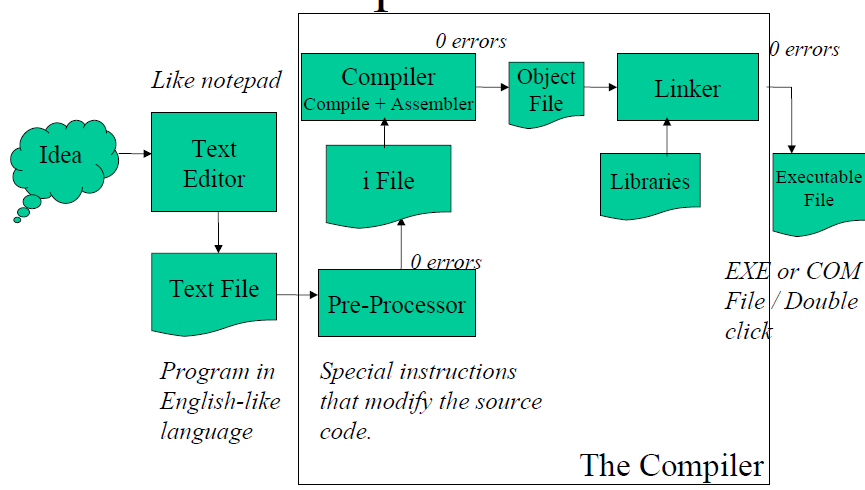
\includegraphics[scale=0.5]{cco}
\paragraph{C Files}
\begin{itemize}
	\item Source files: file.c (program). file.h (header, shared)
	\item Pre-processed: file.i
	\item Object \& assembler: file.o, file.s
	\item Executables: file, a.out
	\end{itemize}
\paragraph{GCC Syntax}
GCC is the GNU C Compiler.
\\ gcc -o executablename sourcefilenames
\\ Variations include:
\begin{itemize}
	\item gcc -E main.c, also make main.i
	\item gcc -S main.c, also make assembler code
	\item gcc -c main.c, also make object code
	\item gcc main.c, make a.out
	\item Extra switches:
	\begin{itemize}
		\item -o filename, specify name of output
		\item -v verbose
		\item -w suppress warnings
		\item -W extra warnings
		\item -Wall all warning messages
		\item -O1 optimize for size and speed
		\item -O2 optimize even more
	\end{itemize}
\end{itemize}
\paragraph{C Types} ~\\
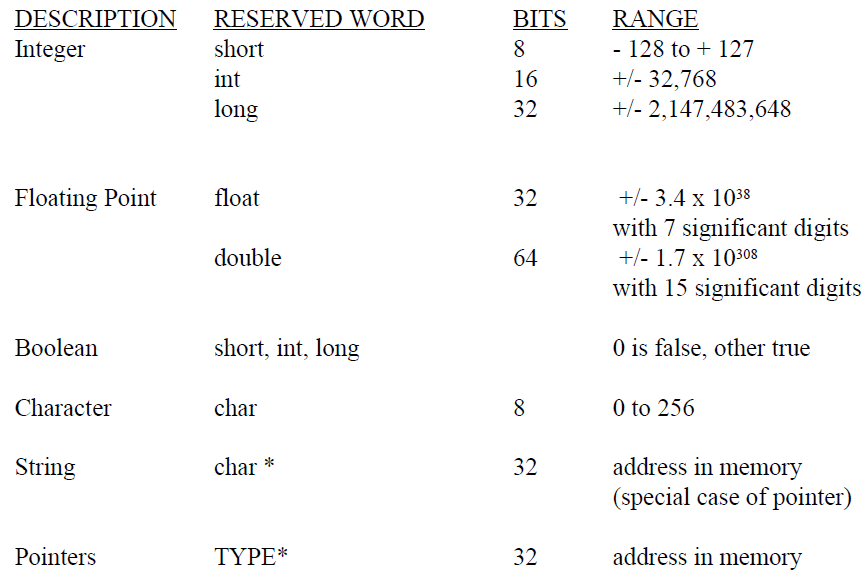
\includegraphics[scale=0.5]{ctyp} Notice that booleans don't really exist (they're just ints) and Strings are char pointers. Strings end with a null.
\paragraph{Booleans}
$0=$ false, anything else is true. Great affects if statements, as your condition can solely be math and it'll check if it's 0 or not. So you won't have a compilation error for something like x=5, but very different from x==5.
\paragraph{Strings} Strings are just character arrays terminated by a null. Can declare some like: char *x = \textquotedbl Bob \textquotedbl;
\\ Cannot scanf into a *, as * constant/fixed to what they were when declared. When scanning into a char array, don't use \&.
\subparagraph{Arrays} int x[10];
\\ Can also declare literally and also leave extra commas to denote extra spaces.
\\ int x[]=\{1,2,3,4,,,,,,\}
\\ In C, you can go past the indexes of an array. 
\\ char x[10]; $\to$ [char][char]$\ldots$[char]
\\ char *y[10]; $\to$ [ptr][ptr]$\ldots$[ptr]
\paragraph{Declaring a Variable}
~\\ SCOPE MODIFIER TYPE VAR\_NAME;
\\ SCOPE is static, extern or not used. MODIFIED is unsigned(no signed bit), short($\frac{1}{2}$ bits), long($2\times $ bits) or not used. TYPE, a built in type.
\\ Variables are \textbf{NOT} defaulted to 0.
\\ Can also chain assignments, int a,b,c,d=4;
\\ Can also declare constants
\\ int const a = 1; or const int a = 2;
\\ Variables declared at either top of file (global variable) or in a function (local variable). Global variables are positionally global, accessible to everything below it. Only one copy of a global variable exists. Global variables should be avoided if not needed, hard to debug and not considered clean.
\\ Variable preference: block vars $\to$ local vars $\to$ global $\to$ extern $\to$ error/compiler error
\subparagraph{typedef Declaration} Can make your own type, i.e.
\\ typedef int boolean;
\subsection{Pointers} Special unsigned integer storing an address. Can reference anything really. Mainly used to point to a variable or location in RAM.
\paragraph{Pointer Operations}
\begin{itemize}
	\item \& unary/monadic operator, gives address of variable
	\item * indirection/dereference, gives contents of object pointed to, declare pointers using *
	\end{itemize}
	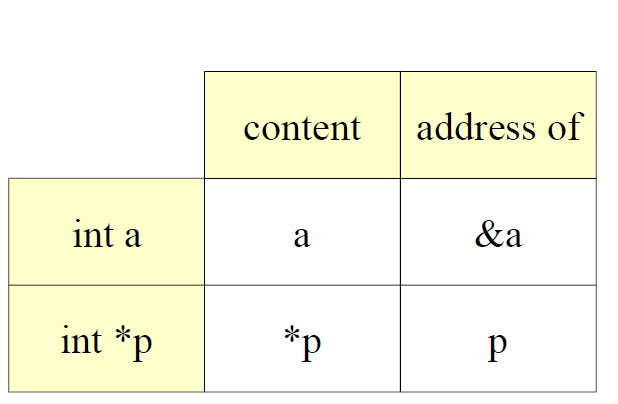
\includegraphics[scale=0.5]{pont}
\begin{lstlisting}[language=c]
int a,b,*p;
p=&a
\end{lstlisting}
p will now point at a's address.
\begin{lstlisting}[language=c]
int a, b;
int *p;

a = 5;
b = 10;
p = &a; // p is pointing to a
*p = 6; // Value of a is now 6
p = &b; // p is pointing to b
*p = 11 // Value of b is now 11;
\end{lstlisting}
Giving type to your pointer means it can only point to that type. void * can point to anything.
\begin{lstlisting}[language=c]
char* x,y,z; // all vars are char*
char x, *y, z; // only y is char*
\end{lstlisting}
Files/text, displayed in 2D but actually 1D structure, like an array. The Disk actually consists of the FAT (File Allocation Table), a bunch of name of files and pointers.
\end{document}